\documentclass[a4paper,ngerman,12pt]{scrartcl}

\usepackage[utf8]{inputenc}
%\usepackage[ansinew]{inputenc}

\usepackage[ngerman]{babel}

\usepackage{amsmath,amsthm,amssymb,stmaryrd,color,graphicx}
\usepackage{setspace}
\usepackage{bussproofs}
\usepackage{array}
\usepackage{comment}
\usepackage{wrapfig}

\usepackage{enumitem}

\usepackage{units}

\usepackage[protrusion=true,expansion=true]{microtype}

\usepackage{lmodern}

\usepackage{hyperref}
\usepackage{cleveref}

\newcommand{\RR}{\mathbb{R}}
\newcommand{\CC}{\mathbb{C}}
\newcommand{\ZZ}{\mathbb{Z}}
\newcommand{\NN}{\mathbb{N}}
\newcommand{\QQ}{\mathbb{Q}}

\setlength\parskip{\medskipamount}
\setlength\parindent{0pt}

\theoremstyle{definition}
\newtheorem{defn}{Definition}[]
\newtheorem{axiom}[defn]{Axiom}
\newtheorem{bsp}[defn]{Beispiel}

\RequirePackage{framed}
\newtheorem{aufg}{Aufgabe}
\definecolor{shadecolor}{rgb}{.96,.96,.96}
\newenvironment{aufgabe}[1][]
		{\begin{shaded}\vspace{-0.3cm}\begin{aufg}\emph{#1} \par\medskip}
		{\end{aufg}\vspace{-0.3cm}\end{shaded}}
	
\newenvironment{spiel}[1][]{\begin{framed}\textbf{#1:}\\}{\end{framed}}


\theoremstyle{plain}
\newtheorem{prop}[defn]{Proposition}
\newtheorem{motto}[defn]{Motto}
\newtheorem{wunder}[defn]{Wunder}
\newtheorem{ueberlegung}[defn]{Überlegung}
\newtheorem{lemma}[defn]{Lemma}
\newtheorem{kor}[defn]{Korollar}
\newtheorem{hilfsaussage}[defn]{Hilfsaussage}
\newtheorem{satz}[defn]{Satz}
\newtheorem{frage}[defn]{Frage}

\theoremstyle{remark}
\newtheorem{bem}[defn]{Bemerkung}

	
\newtheorem*{antwort}{Antwort}

%\newlength{\aufgabenskip}
%\setlength{\aufgabenskip}{1.4em}
%\newcounter{aufgabennummer}
%\newenvironment{aufgabe}[1]{
%	\addtocounter{aufgabennummer}{1}
%	\textbf{Aufgabe \theaufgabennummer.} \emph{#1} \par
%}{\vspace{\aufgabenskip}}

\clubpenalty=10000
\widowpenalty=10000
\displaywidowpenalty=10000

\setlength\unitlength{1cm}

\usepackage{tikz}
\usetikzlibrary{calc}
\usepackage{adjustbox}
\usepackage{algorithm2e}

\RequirePackage{geometry}
\geometry{textwidth=17.0cm,textheight=25cm,footskip=1.5cm}


\newcommand{\kante}[2]{#1{-}#2}
\newcommand{\edge}[3]{\draw[thick] (#1) --node[rectangle,fill=gray!10]{$#3$} (#2);}

\begin{document}
	
\begin{picture}(0,0)
\put(0,-0.5){%
	
\includegraphics[scale=0.1]{logo-ifm}
}
\put(14.0,-3.5){%
	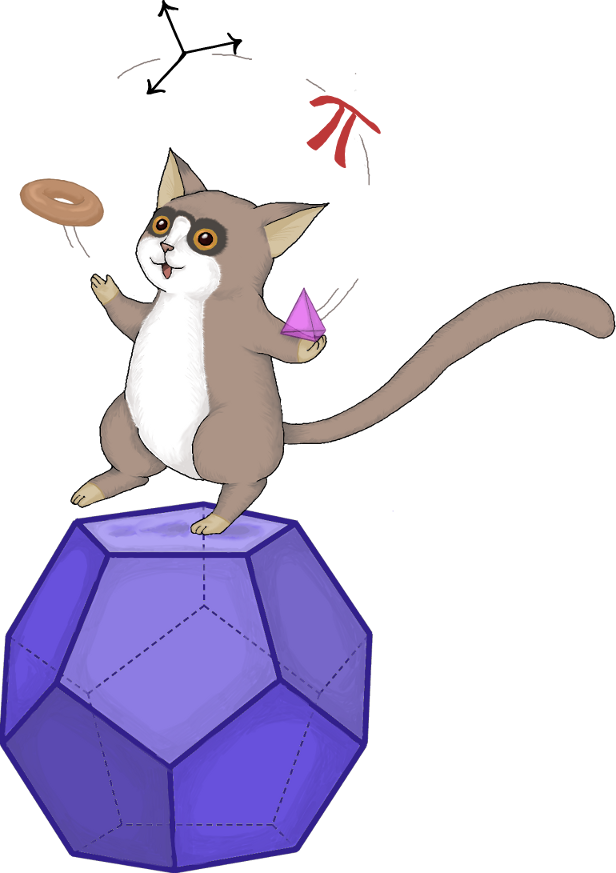
\includegraphics[scale=0.17]{cover}
}
\end{picture} 
	
\vspace{6em}

\begin{center}\Large{Mai-Mathetag 2023}

\section*{Spiele und Gewinnstrategien}\end{center}

\begin{spiel}[Ein einfaches Nim-Spiel]
	Wir starten mit einem Haufen von Münzen. Die beiden Spielerinnen müssen nun abwechselnd eine, zwei, drei oder vier Münzen wegnehmen. Wer die letzte Münze wegnimmt, gewinnt.
\end{spiel}

\begin{aufgabe}
	Spiele das Spiel mit verschiedenen Anzahlen an Münzen zu Beginn. Wenn du zusätzliche Variation willst, kannst du auch eine andere Zahl von Münzen vereinbaren, die man in jedem Zug wegnehmen darf.
\end{aufgabe}

\begin{aufgabe}
	Gibt es für eine der beiden Spielerinnen (die Startspielerin oder die zweite Spielerin) eine \emph{Gewinnstrategie}? Also eine Strategie, mit der sie immer gewinnen kann egal was die andere Spielerin macht?
	
	\textbf{Tipp:} Überlege dir zunächst einmal, was passiert, wenn wir nur mit einer kleinen Zahl von Münzen starten. Also nur mit einer oder zwei oder fünf? Was passiert bei sechs, sieben oder zehn? Findest du ein Muster?
	
	\textbf{Zusatzfrage:} Was ist, wenn die Spielerinnen in jedem Zug bis zu $k$ (für irgendeine feste Zahl $k$) wegnehmen dürfen?
\end{aufgabe}

%% Lösung:
% Startspielerin hat eine Gewinnstrategie, wenn die Zahl der Münzen zu Beginn nicht durch 5 teilbar ist. Dann immer so viele Münzen wegnehmen, dass eine durch 5 teilbare Zahl übrig bleibt.
% Beginnt das Spiel mit einer durch 5 teilbaren Zahl von Münzen hat die zweite Spielerin eine Gewinnstrategie.
% Bei der Zusatzfragee gilt das gleiche für k+1

\newpage
\begin{spiel}[Münzen legen]
	In der Mitte eines runden Tisches liegt eine Münze. Die beiden Spielerinnen legen nun immer abwechselnd je eine weitere Münze auf den Tisch. Die Münzen müssen dabei ganz auf dem Tisch liegen, dürfen sich also nicht mit anderen Münzen überlappen. Wer keine Münze mehr auf den Tisch legen kann, hat verloren.
\end{spiel}

\begin{aufgabe}
	Spiele das Spiel auf dem unten abgebildeten Kreis.
\end{aufgabe}

\begin{center}
	\begin{tikzpicture}[scale=1]
		\node[draw,circle,thick,,minimum size=2cm] () at (0,0){1};
		\node[draw,circle,minimum size=10cm] () at (0,0){};
	\end{tikzpicture}  
\end{center}

\begin{aufgabe}
	Hat eine der beiden Spielerinnen eine Gewinnstrategie? Wenn ja, wie sieht diese aus?
	
	\textbf{Zusatzfrage:} Was passiert, wenn das Spiel mit einem leeren Tisch beginnt?
\end{aufgabe}

%% Lösung: 
% Die zweite Spielerin hat eine Gewinnstrategie: Sie legt ihre Münze immer an die Position, die sie erhält, wenn sie die Position der zuletzt von der Startspielerin platzierten Münze an der mittleren Münze spiegelt.
% Bei der Zusatzfrage hat die Startspielerin eine Gewinnstrategie: Sie beginnt damit ihre erste Münze in die Mitte des Tisches zu legen und verfolgt danach die Gewinnstrategie von zuvor.

\newpage
\begin{spiel}[Plus und Mal]
	Auf einem Blatt Papier stehen in einer Reihe die Zahlen von $1$ bis $10$. Die beiden Spielerinnen platzieren abwechselnd eines der Rechenzeichen $+$ und $\times$ zwischen je zwei Zahlen. Sobald alle neun Lücken mit Rechenzeichen gefüllt sind, berechnet man das Ergebnis der Rechnung. Ist dieses eine ungerade Zahl, so gewinnt die Startspielerin -- andernfalls gewinnt die zweite Spielerin.
\end{spiel}

\begin{aufgabe}
	Spiele das Spiel einige Male. Du kannst auch mit mehr oder weniger Zahlen starten.
\end{aufgabe}

\begin{center}\Large
	\[1 \qquad 2 \qquad 3 \qquad 4 \qquad 5 \qquad 6 \qquad 7 \qquad 8 \qquad 9 \qquad 10 = \]\vspace{.5em}
	\[1 \qquad 2 \qquad 3 \qquad 4 \qquad 5 \qquad 6 \qquad 7 \qquad 8 \qquad 9 \qquad 10 = \]\vspace{.5em}
	\[1 \qquad 2 \qquad 3 \qquad 4 \qquad 5 \qquad 6 \qquad 7 \qquad 8 \qquad 9 \qquad 10 = \]\vspace{.5em}
	\[1 \qquad 2 \qquad 3 \qquad 4 \qquad 5 \qquad 6 \qquad 7 \qquad 8 \qquad 9 \qquad 10 = \]\vspace{.5em}
	\[1 \qquad 2 \qquad 3 \qquad 4 \qquad 5 \qquad 6 \qquad 7 \qquad 8 \qquad 9 \qquad 10 = \]\vspace{.5em}
	\[1 \qquad 2 \qquad 3 \qquad 4 \qquad 5 \qquad 6 \qquad 7 \qquad 8 \qquad 9 \qquad 10 = \]\vspace{.5em}
	\[1 \qquad 2 \qquad 3 \qquad 4 \qquad 5 \qquad 6 \qquad 7 \qquad 8 \qquad 9 \qquad 10 = \]\vspace{.5em}
\end{center}

\begin{aufgabe}
	Hat eine der beiden Spielerinnen eine Gewinnstrategie? Wenn ja, wie sieht diese aus?
\end{aufgabe}

%% Lösung:
% Die Startspielerin hat folgende Gewinnstrategie: Beginne mit einem + zwischen 1 und 2. Danach platziere immer ein x neben der ungeraden Zahl neben der die zweite Spielerin gerade ein Rechenzeichen gesetzt hat (überlege dir, warum das immer möglich ist!). Das führt dazu, dass jede ungerade Zahl mit Ausnahme der 1 mit einer geraden Zahl multipliziert wird. Das Gesamtergebnis ist dann immer 1 + gerade Zahl, also eine ungerade Zahl.

\newpage
\begin{spiel}[Nim mit mehreren Haufen]
	Wir starten mit mehreren Haufen von Münzen. Die beiden Spielerinnen wählen nun abwechselnd einen der Haufen aus und entfernen eine beliege Anzahl von Münzen aus diesem (aber mindestens eine!). Wieder gilt: Wer die letzte Münze wegnimmt, gewinnt.
\end{spiel}

\begin{aufgabe}
	Spiele das Spiel einige Male mit verschieden großen und verschiedenen vielen Haufen zu Beginn.
\end{aufgabe}

\begin{aufgabe}
	Finde möglichst viele Startsituationen, in denen du eine Gewinnstrategie für eine der beiden Spielerinnen angeben kannst. \\
	Kannst du diese Frage vollständig für den Fall beantworten, dass wir das Spiel mit zwei Haufen starten?
\end{aufgabe}

%% Lösung:
% Für zwei Haufen hat die zweite Spielerin eine Gewinnstrategie, wenn die Haufen gleich groß sind: Kopiere jeden Zug der Startspielerin (im jeweils anderen Haufen)
% Sind die beiden Haufen nicht gleich groß, so hat die Startspielerin eine Gewinnstrategie: Mache die beiden haufen im ersten Zug gleich groß und kopiere danach die Züge der zweiten Spielerin.
% Für drei Haufen hat der Startspieler eine Gewinnstrategie, wenn zwei der drei Haufen zu Beginn gleich groß sind.

\begin{aufgabe}
	Auch für mehr als zwei Haufen kann man eine allgemeine Gewinnstrategie beschreiben. Diese zu finden ist allerdings etwas schwieriger und benötigt einen Trick: \\
	Schreibe die Zahl der Münzen in jedem Haufen als Binärzahl. Addiere die so erhaltenen Binärzahlen dann schriftlich aber ohne Übertrag. Nun muss man testen, ob diese \glqq Summe\grqq{} nur aus geraden Zahlen besteht oder nicht. \\
	Führe diesen Trick für die Startsituationen durch, die du in der vorherigen Aufgabe gefunden hast. Fällt dir dabei etwas auf? Kannst du deine Vermutung beweisen?
\end{aufgabe}

%% Lösung:
% Eine Situation ist eine Gewinnsituation, wenn die "Summe" wenigstens eine ungerade Zahl enthält und eine Verlustsituation, wenn die Summe nur gerade Zahlen enthält.

\newpage
\begin{spiel}[Ein Einspielerspiel]
	In diesem Spiel gibt es nur eine Spielerin: Diese startet mit einem karierten Feld mit einer waagrechten Linie in der Mitte. Sie darf nun zunächst beliebig viele Münzen in die Felder unterhalb der waagrechten Linie platzieren (aber immer nur eine Münze pro Feld)! Sobald sie all ihre Münzen platziert hat, beginnt das eigentliche Spiel: Eine Münze kann eine andere überspringen, wenn das entsprechende Feld hinter der zweiten Münze frei ist. Die übersprungene Münze wird danach vom Spielfeld entfernt. Die Spielerin kann diesen Spielzug nun so oft wiederholen bis kein weiterer mehr möglich ist.
	
	Dein Ziel ist es mit wenigsten einer Münze so weit wie möglich oberhalb der waagrechten Linie zu kommen.
\end{spiel}

\begin{aufgabe}
	Spiele das Spiel. Wie hoch schaffst du es? Wie viele Münzen brauchst du dafür?
	
	\textbf{Tipp:} Fange klein an! Versuche erstmal nur ein Feld hoch zu kommen. Dann zwei. Dann drei. Kannst du dieses System fortsetzen?
\end{aufgabe}

\begin{center}
     \begin{tikzpicture}[scale=1]
     	\draw[step=1.5cm] (0,0) grid (16.5,14);
     	\draw[red,ultra thick] (-0.5,7.5) -- (17,7.5);
	\end{tikzpicture}  
\end{center}

\newpage
\begin{aufgabe}
	\textbf{Schwere Bonusaufgabe:} Tatsächlich ist es nicht möglich irgendein Feld der Höhe $5$ zu erreichen -- egal mit wie vielen Münzen man startet. Kannst du das beweisen?
	
	\textbf{Hinweis:} Auf diesen Beweis alleine zu kommen, ist vermutlich zu schwierig (ich musste ihn jedenfalls auch nachlesen!). Du kannst dir aber bei mir ein paar Tipps abholen wie man zu diesem Beweis kommt. Alternativ kannst du dieses sehr schöne (englische) Video anschauen, in dem der Beweis erklärt wird: \url{https://youtu.be/BMPa0FA65Fk}
\end{aufgabe}

%% Lösung:
% 4 ist die maximal erreichbare Höhe - mögliche Startpositionen sind:
% für 1: 
% ---------
%    o
%    o
% für 2: 
% ---------
%    ooo
%    o
% für 3: 
% ---------
%  ooooo
%    ooo
% für 4: 
% ---------
%  ooooooo
%  ooooo
%  oooooo
%    o
% Für mehr Erklärungen und einen Beweis, warum 5 nicht möglich ist siehe https://www.youtube.com/watch?v=BMPa0FA65Fk

\begin{center}
	\begin{tikzpicture}[scale=1]
		\draw[step=.5cm] (0,0) grid (16.5,18);
		\draw[red,ultra thick] (-0.5,11.5) -- (17,11.5);
	\end{tikzpicture}  
\end{center}

\end{document}